\documentclass[10pt,journal,compsoc]{IEEEtran}

\makeatletter
% IEEEtran.cls defines \labelindent for backward compatibility reasons
% Undefine \labelindent to allow the use of package enumitem
\let\labelindent\relax
\makeatother

\ifCLASSOPTIONcompsoc
  % IEEE Computer Society needs nocompress option
  % requires cite.sty v4.0 or later (November 2003)
  \usepackage[nocompress]{cite}
\else
  % normal IEEE
  \usepackage{cite}
\fi

\usepackage[T1]{fontenc}
\usepackage[para]{footmisc}
\usepackage[pdftex]{graphicx}
\usepackage[utf8]{inputenc}
\usepackage{array}
\usepackage{balance}
\usepackage{booktabs}
\usepackage{color}
\usepackage{comment}
\usepackage{enumitem}
\usepackage{framed}
\usepackage{listings}
\usepackage{microtype}
\usepackage{subcaption}
\usepackage{url}


% SQUEEZE
%\addtolength{\parskip}{-1pt}


\definecolor{lightred}{RGB}{150,0,0}
\definecolor{lightgreen}{RGB}{0,150,0}
\definecolor{lightblue}{RGB}{0,0,150}

\lstdefinelanguage{diff}{
  morecomment=[f][\color{lightblue}]{diff },
  morecomment=[f][\color{lightblue}]{index },
  morecomment=[f][\color{lightblue}]{@@},     % group identifier
  morecomment=[f][\color{lightred}]-,         % deleted lines
  morecomment=[f][\color{lightgreen}]+,       % added lines
  morecomment=[f][\color{lightblue}]{---},    % Diff header lines (must appear after +,-)
  morecomment=[f][\color{lightblue}]{+++},
}
\hyphenation{}

\newcommand{\attn}[1]{{\color{red}#1}}
\newcommand{\desc}[1]{{\emph{\color{blue}#1}}}
\newcommand{\needcite}{\attn{\tiny{[cite]}}}
\newcommand{\todo}[1]{\strut\smash{\colorbox{yellow}{\bf TODO: #1}}}
\setlength\OuterFrameSep{0.5em}
\setlength\FrameSep{0.5em}

\begin{document}
\title{Modeling Changeset Topics for Feature Location}
\author{%
    Christopher~S.~Corley
    and~Nicholas~A.~Kraft%
    \thanks{Manuscript received never; revised in my dreams.}}


\markboth{Journal of WOOO}%
{Corley & Kraft: Modeling Changeset Topics for Feature Location}


\IEEEtitleabstractindextext{%
\begin{abstract}
Feature location is a program comprehension activity in which a developer
inspects source code to locate the classes or methods that implement a feature of interest.
Many feature location techniques (FLTs) are based on text retrieval models, and
in such FLTs it is typical for the models to be trained on source code snapshots.
However, source code evolution leads to model obsolescence and
thus to the need to retrain the model from the latest snapshot.
In this paper, we introduce a topic-modeling-based FLT in which the model
is built incrementally from source code history.
By training an online learning algorithm using changesets, the FLT
maintains an up-to-date model without incurring the non-trivial computational cost associated with retraining traditional FLTs.
Overall, we studied over 1,200 defects and features from 14 open-source Java projects.
We also present a historical simulation that demonstrates how the FLT performs as a project evolves.
Our results indicate that the accuracy of a changeset-based FLT is similar to that of a snapshot-based FLT, but without the retraining costs.
\end{abstract}

\begin{IEEEkeywords}
program comprehension,
feature location,
topic modeling,
mining software repositories,
changesets.
\end{IEEEkeywords}
}


\maketitle

\IEEEdisplaynontitleabstractindextext
\IEEEpeerreviewmaketitle

\IEEEraisesectionheading{\section{Introduction}\label{sec:intro}}
% vim:syntax=tex

\IEEEPARstart{F}{eature} location is a frequent and fundamental activity for a developer tasked with changing a software system.
Whether a change task involves adding, modifying, or removing a feature, a developer cannot complete the task without first locating the source code that implements the feature.
The state-of-the-practice in feature location is to use an IDE tool based on keyword or regex search, but Ko et al.~\cite{Ko-etal:2006} observed such tools leading developers to failed searches nearly 90\% of the time.

The state-of-the-art in feature location~\cite{Dit-etal:2011} is to use a feature location technique (FLT) based, at least in part, on text retrieval (TR).
The standard methodology~\cite{Marcus-etal:2004} is to extract a document for each class or method in a source code snapshot, to train a TR model on those documents, and to create an index of the documents from the trained model.
Topics models (TMs)~\cite{Blei:2012} such as latent Dirichlet allocation (LDA)~\cite{Blei-etal:2003} are the state-of-the-art in TR and outperform vector-space models (VSMs) in the contexts of natural language~\cite{Deerwester-etal:1990,Blei-etal:2003} and source code~\cite{Poshyvanyk-etal:2007,Lukins-etal:2010}.
Yet, modern TMs such as online LDA~\cite{Hoffman-etal:2010} natively support only the online addition of a new document, whereas VSMs also natively support online modification or removal of an existing document.
So, TM-based FLTs provide the best accuracy, but unlike VSM-based FLTs, they require computationally-expensive retraining subsequent to source code changes.

Rao\cite{Rao:2013} proposed FLTs based on customizations of LDA and latent semantic indexing (LSI) that support online modification and removal.
%These FLTs require less-frequent retraining than others based on TMs.
These FLTs require less-frequent retraining than other TM-based FLTs,
but the remaining cost of periodic retraining inhibits their application to large software, and the reliance on customization hinders their extension to new TMs.

We envision an FLT that is: (1)~accurate like a TM-based FLT, (2)~inexpensive to update like a VSM-based FLT, and (3)~extensible to accommodate any off-the-shelf TR model that supports online addition of a new document.
Unfortunately, our vision is incompatible with the standard methodology for FLTs.
Existing VSM-based FLTs fail to satisfy the first criteria, and existing TM-based FLTs fail to satisfy the second or third criteria.
Indeed, given the current state-of-the-art in TR, it is impossible for a FLT to satisfy all three criteria while following the standard methodology.

In this paper we propose a new methodology for FLTs.
Our methodology is to extract a document for each changeset in the source code history and to train a TR model on the changeset documents, and then to extract a document for each class or method in a source code snapshot and to create an index of the class/method documents from the trained (changeset) model.
This new methodology stems from four key observations:
\begin{itemize}[leftmargin=*]
  \item
    Like a class/method definition, a changeset has program text.
  \item
    Unlike a class/method definition, a changeset is immutable.
  \item
    A changeset corresponds to a commit.
  \item
    An atomic commit involves a single feature.
\end{itemize}
It follows from the first two observations that it is possible for an FLT following our methodology to satisfy all three of the criteria above.
The next two observations influence the training and indexing steps of our methodology,
which have the conceptual effect of relating classes (or methods) to changeset topics.
By contrast, the training and indexing steps of the standard methodology
have the conceptual effect of relating classes to class topics (or methods to method topics).

To evaluate the new methodology, we used it to implement FLTs based on online LSI and online LDA.
We next used two benchmarks to compare the accuracy of these FLTs to the accuracy of analogous FLTs following the standard methodology.
Combined, the two benchmarks comprise over 1,200 defects and features from 14 open-source Java projects.
We then used a subset of over 600 defects and features to conduct a historical simulation that demonstrates how the FLTs perform as a project evolves.
%Our evaluation results provide evidence that our new methodology is sound and indicate that FLTs following it provide similar accuracy to those following the standard methodology while eliminating retraining costs.
Our evaluation results provide evidence that our new methodology is sound and that following it yields FLTs with similar accuracy to those following the standard methodology, but without the retraining costs.

The remainder of the paper is organized as follows.
We first review background and related work (\S\ref{sec:related})
We next present our new methodology for FLTs (\S\ref{sec:changeset}) and report evaluation results for the online-LDA-based FLT (\S\ref{sec:study}).
We then conclude (\S\ref{sec:conclusion}).




\begin{comment}
Software developers are often confronted with maintenance tasks that involve
navigation of repositories that preserve vast amounts of project history.
Navigating these software repositories can be a time-consuming task, because
their organization can be difficult to understand.  A software developer who is
tasked with changing a large software system spends effort on program
comprehension activities to gain the knowledge needed to make the
change~\cite{Corbi:1989}.  Fortunately, topic models such as latent Dirichlet
allocation (LDA)~\cite{Blei-etal:2003} can help developers to navigate and
understand software repositories by discovering topics (word distributions) that
reveal the thematic structure of the
data~\cite{Linstead-etal:2007,Thomas-etal:2011,Hindle-etal:2014}.

One particular application of topic models is for \emph{feature location}.
Feature location is the act of identifying the source code that implements
a system feature.  The current state-of-the-practice for feature location is to
use a keyword search tool, such as \texttt{grep}.  Ko et al.~\cite{Ko-etal:2006}
show that developers fail using this type of searching upwards to 88\% of the
time.  Text retrieval techniques, such as topic modeling, show promise in
remedying this problem~\cite{Marcus-etal:2004}.

Typical topic-modeling-based feature location techniques (FLT) construct models
from corpora of text extracted from a source code snapshot~\cite{Dit-etal:2011}.
To use a topic-modeling-based FLT, there are generally two key steps: training
and indexing.  In the first step, a corpus of source code entities, such as
methods or classes, are used to train the model to learn word co-occurences
within those entities.  The indexing step uses the trained model to construct an
index of the source code entities based on their inferred topic distribution.
That is, an index is made of each source code's \emph{thematic structure}, and
not it's raw content.  Keeping such a model and index up-to-date is expensive,
because the frequency and scope of source code changes, such as file removal,
necessitate retraining the model on the updated corpus and reindexing.  This
situation is sub-optimal whether your perspective is academic research or
industrial tool-building.  Like Rao et al.~\cite{Rao-etal:2013}, our primary
research goal is elimination of this cost.  However, unlike Rao et al., we do
not intend to develop new topic modeling techniques, but rather use the existing
ones.

In this paper, we propose a fresh take on topic-modeling-based FLTs by
leveraging online topic models and mining software repositories to construct
topic models that do not need retraining.  Online topic models do not need to
know the entire input corpus prior to
training~\cite{Hoffman-etal:2010}.  That is, online topic models can
be incrementally trained over time as more data becomes available.
Moreover, a version control repository, such as Git, keeps a history of source
code documents as they change over time.  These changes are represented as
changesets, which provide concise views of the differences between two revisions
of the same document.  By training an online topic model on changesets and
indexing the source code on that model, we can stream documents (i.e.,
changesets) from the version control repository to incrementally train the topic
model.  This enables searching over the current source code index without
retraining an entirely new model.

In our previous work~\cite{Corley-etal:2014}, we show that topic models trained
on changesets produce topics which have comparable topic distinctness
scores~\cite{Thomas-etal:2011} as topic models trained on snapshots.  Further,
we show that the corpora express the same frequency of words.  We expand the
work to demonstrate the effectiveness of changeset topic modeling for feature
location and report on an empirical study in which we investigate the
feasibility of this approach.
We define a LDA-based FLT using changesets.  We combine two benchmarks totaling
over 1200 defects and features from fourteen open source Java projects.  We also
present a \emph{historical simulation} that approximates how the FLT would perform
throughout the evolution of a project.

Our results show that the changeset approach is feasible and has performace
comparable to the snapshot approach.  In many cases the changeset approach
out-performs current snapshot approach, but is no silver bullet.  We argue
that the evidence suggests that changeset-based topic modeling warrants further
investigation and adoption.  Additionally, the historical simulation suggests that
current evaluation approaches do not accurately capture the true FLT
performance.

This paper makes the following contributions:

\begin{itemize} \item An approach for using changesets for feature location
        \item A empirical study of fourteen open source Java projects \item
            Towards increasing open science principles in software engineering:
            the complete project history, source code, and an updated dataset
            for replication of this study.  \end{itemize}

The remainder of the paper is organized as follows.  We first review background
and related work (\S\ref{sec:related}) before introducing our new
changeset-based FLT (\S\ref{sec:changeset}).  We next discuss our case study
(\S\ref{sec:study}), which spans fourteen open source Java projects.  We then
conclude (\S\ref{sec:conclusion}).
\end{comment}



\section{Background \& Related Work}
\label{sec:related}
% vim:syntax=tex

\begin{figure*}[t]
    \centering
\begin{subfigure}[t]{.9\textwidth}
    \centerline{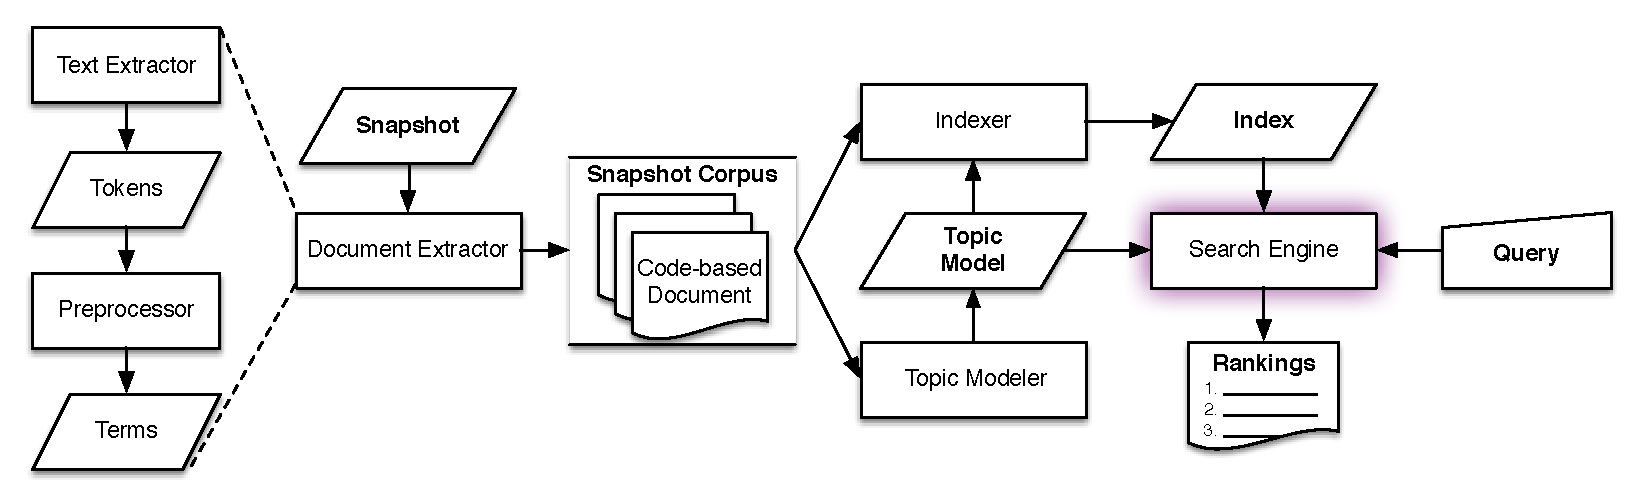
\includegraphics[width=\textwidth]{figures/snapshot-flt}}
    \caption{Topic-modeling-based feature location technique using snapshots}
    \label{fig:snapshot}
\end{subfigure}

\begin{subfigure}[b]{.9\textwidth}
    \centerline{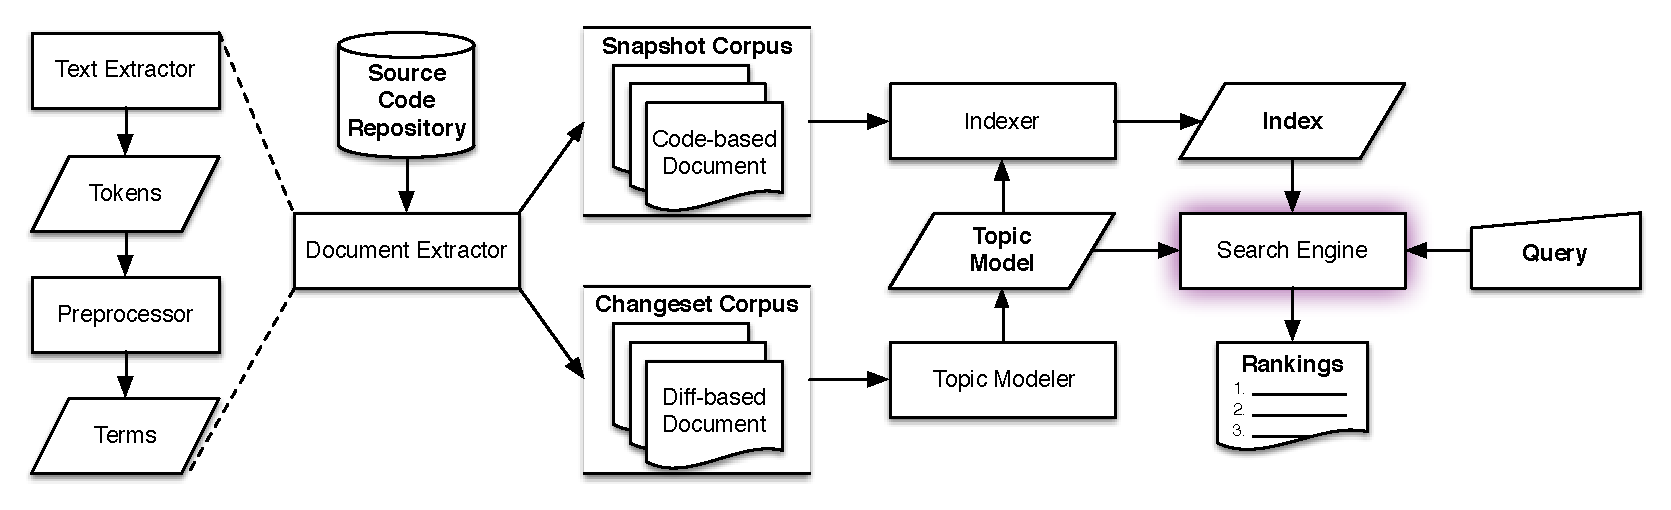
\includegraphics[width=\textwidth]{figures/changeset-flt}}
\caption{Topic-modeling-based feature location technique using changesets}
\label{fig:changeset}
\end{subfigure}

\label{fig:flts}
\caption{Two feature location techniques side-by-side}
\end{figure*}


In this section, we review the standard methodology for document extraction and
retrieval process used by snapshot-based FLTs, as well as related work on topic
modeling and feature location.

\subsection{Document Extraction and Retrieval Process}
\label{sec:snapshot-flt}

We use the following terminology to describe document extraction of a source code snapshot.
A \textit{word} is the basic unit of discrete data in a software lexicon and is a sequence of letters.
A \textit{token} is a sequence of non-whitespace characters containing one or more words.
An \textit{entity} is a named source element such as a method,
and an \textit{identifier} is a token representing the name of an entity.
\textit{Comments} and \textit{literals} are sequences of tokens delimited by language-specific markers (e.g., /* */ and quotes).
The \textit{document} which corresponds to an entity is a sequence of words $d = (w_1, \ldots, w_m)$,
and a \textit{corpus} is a set of documents (i.e., methods) $D = (d_1, \ldots, d_n)$.

The left side of Figure~\ref{fig:snapshot} illustrates the document extraction
process.  A document extractor takes a source code snapshot as input and produces a corpus
as output.  Each document in the corpus contains the words associated with
a source code entity, such as a class or method.  The text extractor is the first
part of the document extractor and parses the source code to produce a token
stream for each document.  The preprocessor is the second part of the document
extractor.  It applies a series of transformations to each token and produces
one or more words from the token.
The transformations commonly used are~\cite{Marcus-etal:2004,Marcus-Menzies:2010}: % that we use are:
\begin{itemize}
    \item {\it Splitting}: separate tokens into constituent words based on
        common coding style conventions (e.g., the use of camel case or
        underscores) and on the presence of non-letters (e.g., punctuation or
        digits)
    \item {\it Normalizing}: replace each upper case letter with the
        corresponding lower case letter
    \item {\it Filtering}: remove common words such as articles (e.g., `an' or
        `the'), programming language keywords, standard library entity names, or
        short words
\end{itemize}

The right side of Figure~\ref{fig:snapshot} illustrates the retrieval process.
The main prerequisite of the retrieval process is to build the search engine.
The search engine is constructed from a topic model trained from a corpus and an
index of that corpus inferred from that model.
This means that an index is no more than each input document's thematic
structure (i.e., the document's inferred topic distribution).

The primary function of the search engine is to rank documents in relation to
the query~\cite{Croft-etal:2010}.  First, when using a TM-based approach, the
engine must first infer the thematic structure of the query.  This allows for
a pairwise classification of the query to each document in the index and ranks
the documents based on the similarities of their thematic structures.

\subsection{Latent Dirichlet Allocation}

LDA~\cite{Blei-etal:2003} is a generative topic model.
LDA models each document in a corpus of discrete data as a finite mixture over
a set of topics and models each topic as an infinite mixture over a set of
topic probabilities.  That is, LDA models each document as a probability
distribution indicating the likelihood that it expresses each topic and models
each topic that it infers as a probability distribution indicating the
likelihood of a word from the corpus being assigned to the topic.

Hoffman et al.~\cite{Hoffman-etal:2010} introduce \textit{online LDA}, an online version of LDA.
Online LDA allows the model to be updated incrementally without
needing to know about the documents prior to model construction.  Zhai and
Boyd-Graber~\cite{Zhai-Boyd-Graber:2013} introduce an extension of LDA in which
the model also does not need to know about the corpus vocabulary prior to
training. Teh et al.~\cite{Teh-etal:2006} introduce an LDA counterpart,
the Hierarchical Dirichlet process (HDP), that learns the appropriate number of
topics from the data, rather than needing configuration. Further, Wang et
al.~\cite{Wang-etal:2011} further extend HDP to bring the algorithm online.


\subsection{Feature Location}

Feature location is the act of identifying the source code entity or entities
that implement a feature~\cite{Rajlich-Wilde:2002}.
%  Bug localization can be seen as the process of identifying source code entities that implement an \emph{unwanted} feature~\cite{Lukins-etal:2010}.
%also target the problem of building topic models, introducing an incremental
%framework for bug localization.  Although practical, the approach involves using
%an extended topic modeler to allow updating, adding, and removing documents from
%the model and index post-hoc.  While the approach is essentially equivalent to
%topic modeling in batch, Rao~\cite{Rao:2013} notes that these algorithm
%modifications have limitations and thus models may need to be periodically
%retrained.
Dit et al.~\cite{Dit-etal:2011} provide a taxonomy and survey of feature
location in source code covering the scope of FLTs.  They identify 89 works
related to feature location in their systematic literature survey and extract
7 dimensions for their taxonomy.  The primary dimension, type of analysis, can
be used for categorization purposes and consists of four categories: dynamic,
static, historical, and textual.
%Dynamic FLTs use information from a system's execution, such as stack
%traces~\cite{Moreno-etal:2014}.  Static FLTs instead use semantic information
%extracted directly from source code, such as method call
%graphs~\cite{Saul-etal:2007}. 
%Historical FLTs~\cite{Cubranic-etal:2005} mine software repositories
%to extract meaningful information
%Textual FLTs use textual information extracted
%from software artifacts, such as source code comments, identifiers, and
%literals~\cite{Biggers-etal:2014}.
%Textual FLTs are the most closely related
%category of our work and comprise the remainder of this section.
Our methodology uses historical analysis (e.g., \cite{Cubranic-etal:2005}) and textual analysis (e.g., \cite{Marcus-etal:2004}).

The most relevant FLTs, by Rao~\cite{Rao-etal:2013, Rao:2013}, are described in the introduction.
Other closely related work involves LSI-based FLTs~\cite{Marcus-etal:2004,Poshyvanyk-etal:2006,Poshyvanyk-Marcus:2007,Liu-etal:2007,Scanniello-Marcus:2011,Cubranic-etal:2005} or LDA-based FLTs~\cite{Lukins-etal:2008,Lukins-etal:2010,Biggers-etal:2014,Bassett-Kraft:2013}.

% Currently, developers rely on tools such as \texttt{grep} to find relevant
% source code entities. Petrenko et al.~\cite{Petrenko-etal:2008} develop
% a \texttt{grep}-based FLT. However, Ko et al.~\cite{Ko-etal:2006} show that
% developers fail using this type of searching upwards to 88\% of the time.  Text
% retrieval techniques, such as topic modeling, show promise in remedying this
% problem~\cite{Marcus-etal:2004}.


% Marcus et al~\cite{Marcus-etal:2004} use an FLT based on Latent Semantic
% Indexing (LSI)~\cite{Deerwester-etal:1990} to find concepts based on queries
% from the user, and modules within the system in comparison to the dependence
% graph approach. They found that concepts in the code were able to be identified
% with user specified terms and identifiers as well as an easier build process.
% LSI-based FLTs have been widely used by many others~\cite{ Poshyvanyk-etal:2006,
% Poshyvanyk-Marcus:2007, Liu-etal:2007, Scanniello-Marcus:2011, % Eaddy-etal:2008,
% Cubranic-etal:2005}.

% Lukins et al.~\cite{Lukins-etal:2008} introduce an FLT based on LDA and find
% that it outperforms an LSI-based FLT.  Biggers et al.~\cite{Biggers-etal:2014}
% investigate the various configuration parameters for an LDA-based FLT.  Bassett
% and Kraft~\cite{Bassett-Kraft:2013} find that using structural term weighting
% increases the performance of an LDA-based FLT.

\subsection{Modeling Software Repositories}

Our work is also not the first to investigate ways to employ topic models on
software repositories. Thomas et al.~\cite{Thomas-etal:2011} present a study on
how topics of a software project evolve over time. They present the \emph{Diff}
model, and closely resembles our work. However, their Diff model is much more
coarse-grained and trains a topic model on changesets between two software
snapshots, not changesets between two commits. Additionally, their goal in using
this model is for modeling the evolution of topics, not for feature location.

Hindle et al.~\cite{Hindle-etal:2009} present a technique that relates
commits to requirements documents using LDA.  They apply LDA to extract
topics from issue reports, requirements documents, and commit messages.  Their
linking process relies on LDA inferencing to derive the topics of unseen documents.
Hindle et al.~\cite{Hindle-etal:2014} use a similar approach.
Our methodology is based on the same inferencing concept and
creates an index of source code entities from learned changeset topics.


\section{Modeling Changeset Topics}
\label{sec:changeset}
% vim:syntax=tex

In this section we describe how a TM-based FLT can use changesets.

\subsection{Terminology}

In addition to the terminology described in Section~\ref{sec:related}, we use
the following terminology to describe the document extraction and retrieval
process of changesets.

A \textit{diff} is a set of text which represents the differences between two texts.
A \textit{patch} is a set of instructions (i.e., diffs) that is used to transform one set of texts into another.
\textit{Context lines} denote text useful for transforming the text, but do not represent the differences.
\textit{Added lines} are lines which were added in order to transform the first text into the second.
Similarly, \textit{removed lines} are lines which are removed for this same purpose.
A \textit{changeset}, ideally, represents a single feature modification,
addition, or deletion, which may crosscut many source code entities.
A \textit{commit} is a representation of a changeset in a version control system, such as Git or Subversion.
Figure~\ref{fig:diff} shows an example changeset from Git.


\begin{figure*}[t]
\centering
\footnotesize
\begin{lstlisting}[language=diff, basicstyle=\ttfamily]
diff --git a/src/java/net/sf/jabref/EntryEditor.java b/src/java/net/sf/jabref/EntryEditor.java
index 8c56723..6b4788e 100644
--- a/src/java/net/sf/jabref/EntryEditor.java
+++ b/src/java/net/sf/jabref/EntryEditor.java
@@ -669,7 +669,8 @@ public class EntryEditor extends JPanel implements VetoableChangeListener {
     public void storeCurrentEdit() {
         Component comp = Globals.focusListener.getFocused();
         if ((comp == source) || ((comp instanceof FieldEditor) && this.isAncestorOf(comp))) {
-            ((FieldEditor)comp).clearAutoCompleteSuggestion();
+            if (comp instanceof FieldEditor)
+                ((FieldEditor)comp).clearAutoCompleteSuggestion();
             storeFieldAction.actionPerformed(new ActionEvent(comp, 0, ""));
         }
     }
\end{lstlisting}
\caption{Example of a \texttt{git diff}.
This changeset addresses JabRef's Issue \#2904968.
Black or blue lines denote metadata about the change useful for patching.
In particular, black lines represent context lines (beginning with a single space).
Red lines (beginning with a single~\texttt{-}) denote line removals,
and green lines (beginning with a single~\texttt{+}) denote line additions.}
\label{fig:diff}
\vspace{-10pt}
\end{figure*}

\subsection{Feature location using changesets}

The overall difference in our methodology and the standard methodology described in Section~\ref{sec:snapshot-flt} is minimal.
For example, compare Figures~\ref{fig:snapshot}~and~\ref{fig:changeset}.
In the changeset approach, we only need to replace the documents on which the topic model is trained
while the remainder of the approach remains the same.
%Our work can be viewed as a hybrid of textual and historical analyses
%under the Dit et al.~\cite{Dit-etal:2011} taxonomy.
% % already mentioned elsewhere


The changeset approach requires two types of document extraction:
the snapshot of the state of source code at a commit of interest, such as
a tagged release, and every changeset in the source code history leading up to
the same commit of interest.  The left side of Figure~\ref{fig:changeset}
illustrates the dual-document extraction approach.

The document extraction process for the snapshot remains the same as covered in
Section~\ref{sec:related} while the document extractor for the changesets parses
each changeset for the removed, added, and context lines.  From there, each line
is tokenized by the text extractor.  The same preprocessor transformations as
before occur in both the snapshot and changesets.  The snapshot vocabulary is
always a subset of the changeset vocabulary~\cite{Corley-etal:2014}.

The right side of Figure~\ref{fig:changeset} illustrates the retrieval process.
The key intuition to our methodology is that a topic model such as LDA or LSI can
infer \emph{any} document's topic proportions regardless of the documents used
to train the model.  In fact, this is also what determining the topic
proportions of a user-created query relies on. Likewise, so are other unseen
documents. In our approach, the seen documents are changesets and the unseen
documents are the source code entities of the snapshot.

Hence, we train a topic model on the changeset corpus and use the model to index
the snapshot corpus.  Note that we never construct an index of the changeset
documents on which the model is trained.  In our approach, we only use the
changesets to continuously update the topic model and only use the snapshot for
indexing.

To leverage the online functionality of the topic models, we can also intermix
the model training, indexing, and retrieval steps.  First, we initialize a model
in online mode.  Then, as changes are made, the model is updated with the new
changesets as they are committed.  That is, with changesets, we incrementally
update a model and can query it at any moment.  Our historical simulation
(\S~\ref{sec:methodology}) relies on this insight.

% In the search engine we can use a dynamic programming to keep the index
% up-to-date as new changesets are added to the model.  That is, upon a update
% to the model, updates to the index are made only to the documents that are
% affected by the changesets.


\subsection{Why changesets?}

We choose to train the model on changesets, rather than another source of
information, because they also represent what we are primarily interested in:
program features.  A single changeset provides text of an addition, removal, or
modification of a single feature.  A developer can to some degree comprehend
what a changeset accomplishes by examining it, such as during a code review,
much like examining a source file directly.

While a snapshot corpus has documents that represent a program, a changeset
corpus has documents that represent programming.  If we consider every changeset
affecting a particular source code entity, then we gain a sliding-window view of
that source code entity over time and the contexts those changes were performed
in.  This is akin to summarizing code snippets with machine
learning\cite{Ying-Robillard:2013}, where in our case a changeset gives
a snippet-like view of the code required to complete a task.  For example, in
Figure~\ref{fig:diff}, we can see the entire method being changed when the
context lines are considered.

Additionally, Vasa et al.~\cite{Vasa-etal:2007} observe that code rarely changes
as software evolves. The implication is that the topic modeler will see
changesets containing the same source code entity only a few times, perhaps only
once.  Since topic modeling a snapshot only sees an entity once, topic modeling
a changeset can miss no information.

Using changesets also implies that the topic model may gain some noisy
information from these additional documents, especially removals.  However, Vasa
et al.\ also observe that code is less likely to be removed than it is to be
changed. This implies that the noisy information would likely remain in both
snapshot-based models and changeset-based models.

Indeed, it appears desirable to remove changesets from the model that are old
and no longer relevant to the current snapshot of the system. There would be no
need for this because online LDA already contains features for increasing the
influence newer documents have on the model, thereby decaying the effect of the
older documents on the model.




\section{Study}
\label{sec:study}
% vim:syntax=tex

In this section we describe the design of a study in which we compare our new
methodology with the current practice. We describe the case study using the
Goal-Question-Metric approach~\cite{Basili-etal:94}.  We discuss the results of
using LDA as our topic modeler, and exclude the LSI discussion for brevity.
Further, the data and source code for the full case study is available in this
paper's online appendix\footnote{\url{http://christop.club/x/cfl/}}.

\subsection{Definition and Context}

% TODO
Our \textit{goal} is to evaluate the effectiveness of TM-based FLTs trained
on changesets.  The \textit{quality focus} of the study is on informing
development decisions and policy changes that could lead to software with fewer
defects.  The \textit{perspective} of the study is of a researcher, developer,
or project manager who wishes to gain understanding of the concepts or features
implemented in the source code.  The \textit{context} of the study spans the
version histories of 14 open source systems.

Toward the achievement of our goal, we pose the following research questions:
\begin{description}[font=\itshape\mdseries,leftmargin=10mm,style=sameline]
    \item[RQ1] Is a changeset-based FLT as accurate as a snapshot-based FLT?
\end{description}

With our new methodology, we also gain the opportunity to simulate how the FLT
would perform in a real development environment, an evaluation technique
not previously feasible due to the run-time of the experiment.

\begin{description}[font=\itshape\mdseries,leftmargin=10mm,style=sameline]
    %\item[RQ2] Are FLTs accurately evaluated in realistic contexts?
    \item[RQ2] Does the accuracy of a changeset-based FLT fluctuate as a project evolves?
\end{description}

At a high level, our goal is to determine the feasibility of using changesets
to train topic models for feature location, especially in realistic development scenarios.

In the remainder of this section we introduce the subjects of our study,
describe the setting of our study, our data collection and analysis procedures,
and report the results of the study using LDA.

%%%%%%%%%%%%%%%%%%%%%%%%%%%%%%%%%%%%%%%%%%%%%%%%%%%%%%%%%%%%%%%%%%%%%%%%

\subsection{Subject software systems}

All of our subject software systems come from two publicly-available datasets.
The first is a dataset of six software systems by Dit et al.~\cite{Dit-etal:2013} and contains method-level goldsets.
This dataset was automatically extracted from changesets that relate to the queries (issue reports).
The second is a dataset of 14 software systems by Moreno et al.~\cite{Moreno-etal:2014} and contains class-level goldsets.
This dataset was automatically extracted from patches attached to issue reports.
The six software systems in the first dataset also appear in the second,
supplying us with both class- and method-level goldsets for the queries.

\begin{table}[t]
\renewcommand{\arraystretch}{1.3}
\footnotesize
\centering
\caption{Subject Systems and Goldset Sizes}
\begin{tabular}{lrrr}
    \toprule
    Subject System     & Features & Classes & Methods \\
    \midrule
    ArgoUML v0.22      & 91       & 287     & 701     \\
    ArgoUML v0.24      & 52       & 154     & 357     \\
    ArgoUML v0.26.2    & 209      & 706     & 1560    \\
    BookKeeper v4.1.0  & 40       & 152     &         \\
    Derby v10.7.1.1    & 32       & 55      &         \\
    Derby v10.9.1.0    & 95       & 410     &         \\
    Hibernate v3.5.0b2 & 20       & 53      &         \\
    Jabref v2.6        & 39       & 131     & 280     \\
    jEdit v4.3         & 150      & 361     & 748     \\
    Lucene v4.0        & 35       & 103     &         \\
    Mahout v0.8        & 30       & 159     &         \\
    muCommander v0.8.5 & 92       & 303     & 717     \\
    OpenJPA v2.0.1     & 35       & 82      &         \\
    OpenJPA v2.2.0     & 18       & 53      &         \\
    Pig v0.8.0         & 85       & 442     &         \\
    Pig v0.11.1        & 48       & 129     &         \\
    Solr v4.4.0        & 55       & 189     &         \\
    Tika v1.3          & 18       & 34      &         \\
    ZooKeeper v3.4.5   & 80       & 285     &         \\
    \midrule
    Total              & 1224     & 4088    & 4363    \\
    \bottomrule
\end{tabular}
\label{table:subjects}
\end{table}

ArgoUML is a UML diagramming tool\footnote{\url{http://argouml.tigris.org/}}.
BookKeeper is a distributed logging service\footnote{\url{http://zookeeper.apache.org/bookkeeper/}}.
Derby is a relational database management system\footnote{\url{http://db.apache.org/derby/}}.
Hibernate is a object/relational mapping framework\footnote{\url{http://hibernate.org/}}.
jEdit is a text editor\footnote{\url{http://www.jedit.org/}}.
JabRef is a BibTeX bibliography management tool\footnote{\url{http://jabref.sourceforge.net/}}.
Lucene is an information retrieval library\footnote{\url{http://lucene.apache.org/core/}}.
Mahout is a tool for scalable machine learning\footnote{\url{https://mahout.apache.org/}}.
muCommander is a cross-platform file manager\footnote{\url{http://www.mucommander.com/}}.
OpenJPA is object/relational mapping tool\footnote{\url{http://openjpa.apache.org/}}.
Pig is a platform for analyzing large datasets\footnote{\url{http://pig.apache.org/}}.
Solr is a search platform\footnote{\url{http://lucene.apache.org/solr/}}.
Tika is a toolkit for extracting metadata and text from various types of files\footnote{\url{http://tika.apache.org/}}.
ZooKeeper is a tool that works as a coordination service to help build distributed applications\footnote{\url{http://zookeeper.apache.org/bookkeeper/}}.


%%%%%%%%%%%%%%%%%%%%%%%%%%%%%%%%%%%%%%%%%%%%%%%%%%%%%%%%%%%%%%%%%%%%%%%%

\subsection{Methodology}
\label{sec:methodology}

For snapshots, the process is straightforward and corresponds to
Figure~\ref{fig:snapshot}.  First, we train a model on the snapshot corpus using
batch training.  That is, the model can see all documents in the corpus at once.
Then, we infer an index of topic distributions with the snapshot corpus.  For
each query in the dataset, we infer the query's topic distribution and rank each
entity in the index with pairwise comparisons.

\begin{comment}
\begin{enumerate}
    \item Build model from the snapshot corpus in batch mode
    \item Infer a $\theta_{Snapshot}$ from the snapshot corpus
    \item Infer a $\theta_{Queries}$ from the query corpus
    \item Classify, or rank, the results from both $\theta$s
\end{enumerate}
\end{comment}


In terms of changesets, the process varies slightly from a snapshot approach, as
shown in Figure~\ref{fig:changeset}.  First, we train a model of the changeset
corpus using batch training.  Second, we infer an index of topic distributions
with the snapshot corpus.  Note that we \emph{do not} infer topic distributions
with the changeset corpus on which the model was built.  Finally, for each query
in the dataset, we infer the query's topic distribution and rank each entity in
the snapshot index with pairwise comparisons.

\begin{comment}
\begin{enumerate}
    \item Build model from the changeset corpus in batch mode
    \item \emph{Do not} infer a $\theta_{Changesets}$
    \item Infer a $\theta_{Snapshot}$ from the snapshot corpus
    \item Infer a  $\theta_{Queries}$ from the query corpus
    \item Classify, or rank, the results from both $\theta$s
\end{enumerate}
\end{comment}


For the historical simulation, we take a slightly different approach.  We first
determine which commits relate to each query (or issue) and partition
mini-batches out of the changesets.  We then proceed by initializing a model for
online training.  Using each mini-batch, or partition, we update the model.
Then, we infer an index of topic distributions with the snapshot corpus at the
commit the partition ends on.  We also obtain a topic distribution for each
query related to the commit.  For each query, we infer the query's topic
distribution and rank each entity in the snapshot index with pairwise
comparisons. Finally, we continue by updating the model with the next
mini-batch.

\begin{comment}
\begin{enumerate}
    \item Initialize a model in online mode
    \item Determine which changesets relate to an issue and partition mini-batches out of the changesets
    \item For each mini-batch:
        \begin{enumerate}
            \item Update the model with mini-batch
            \item Update $\theta_{Snapshot}$ with the new inference of the source code document affected by this changeset
            \item Infer a $\theta_{Query}$ of the query related to the changeset we stopped at
            \item Classify, or rank, the results from both $\theta$s
        \end{enumerate}
\end{enumerate}
\end{comment}

Since the Dit et al. dataset was extracted from the commit that implemented the
change, our partitioning is inclusive of that commit.  That is, we update the
model with the linked commit and infer the snapshot index from that commit.
This allows our evaluations to capture any entities added to address the issue
report, as well as changed entities, but does not capture any entities that were
removed by the change.



%%%%%%%%%%%%%%%%%%%%%%%%%%%%%%%%%%%%%%%%%%%%%%%%%%%%%%%%%%%%%%%%%%%%%%%%

\subsection{Setting}

Our document extraction process is shown on the left side of Figure~\ref{fig:changeset}.
We implemented our document extractor in Python v2.7
using the Dulwich library\footnote{\url{http://www.samba.org/~jelmer/dulwich/}}
for interacting with the source code repository and
Taser\footnote{\url{https://github.com/nkraft/taser}} for parsing source code.
We extract documents from both a snapshot of the repository at a tagged
snapshot and each commit reachable from that tag's commit.
The same preprocessing steps are employed on all documents extracted.

For our document extraction from a snapshot, we first parse each Java file using our tool, Taser, which
is a text extractor implemented in Java using an open source Java 1.5 grammar and ANTLR v3.
The tool extracts documents from the chosen source code entity type, either methods or classes.
We consider interfaces, enumerations, and annotation types to also be a class.
The text of inner an entity (e.g., a method inside an anonymous class)
is only attributed to that entity, and not the containing one.
Comments, literals, and identifiers within a entity are considered as text of the entity.
Block comments immediately preceding an entity are also included in this text.

To extract text from the changesets, we look at
the \texttt{git diff} between two commits.
In our changeset text extractor, we extract all text related to the
change, e.g., context, removed, and added lines; metadata lines are ignored.
Note that we do not consider where the text originates from,
only that it is text changed by the commit.%\footnote{
%The Apache Lucene and Solr projects were merged into a single, new repository
%during their development.
%We only use changes that affect each project's subdirectory in the merged repository,
%and also include all changes from the two pre-merge repositories in each project's respective corpus.
%}

After extracting tokens, we split the tokens based on camel case,
underscores, and non-letters.
We only keep the split tokens; original tokens are discarded.
We normalize to lower case before filtering non-letters, English stop words~\cite{StopWords}, Java keywords, and words shorter than three characters long.
We do not stem words.

We implemented our modeling using the Python library Gensim~\cite{Gensim},
version 0.10.3. We use the same configurations on each subject system.  We do
not try to adjust parameters between the different systems to attempt to find
a better, or best, solution; rather, we leave them the same to reduce
confounding variables.  We do realize that this may lead to topic models that
may not be best-suited for feature location on a particular subject system.
However, this constraint gives us confidence that the measurements collected are
fair and that the results are not influenced by selective parameter tweaking.
Again, our goal is to show the performance of the changeset-based FLT against
snapshot-based FLT under the same conditions.

Gensim's LDA implementation is based on an online LDA by Hoffman et
al.~\cite{Hoffman-etal:2010} and uses variational inference instead of
a collapsed Gibbs sampler.  Unlike Gibbs sampling, in order to ensure that the
model converges for each document, we allow LDA to see each mini-batch $5$ times
by setting Gensim's initialization parameter \texttt{passes} to this value and
allowing the inference step $1000$ iterations over a document.  We set the
following LDA parameters for all 14 systems: $500$ topics ($K$), a symmetric
$\alpha=1/K$, and a symmetric $\eta=1/K$.  These are default values for
$\alpha$ and $\eta$ in Gensim.

For the historical simulation, we found it beneficial to consider two other
parameters: $\kappa$ and $\tau_0$.  As noted in Hoffman et
al.~\cite{Hoffman-etal:2010}, it is beneficial to adjust $\kappa$ and $\tau_0$
to higher values for smaller mini-batches.  These two parameters control how
much influence a new mini-batch has on the model when training.  We follow the
recommenations in Hoffman et al.\, choosing $\tau_0=1024$ and $\kappa=0.9$ for
all systems, because the historical simulation often has mini-batch sizes in
single digits.


%%%%%%%%%%%%%%%%%%%%%%%%%%%%%%%%%%%%%%%%%%%%%%%%%%%%%%%%%%%%%%%%%%%%%%%%


\subsection{Data Collection and Analysis}
\label{sec:data}

To evaluate the performance of a TM-based FLT we cannot use
measures such as precision and recall. This is because the FLT creates
the rankings pairwise, causing every entity being searched to appear in the rankings.
Poshyvanyk et al. define an effectiveness measure that can be used for TM-based FLTs~\cite{Poshyvanyk-etal:2007}.
The effectiveness measure is the rank of the first relevant document
and represents the number of source code entities a developer would have to view before reaching a relevant one.
The effectiveness measure allows evaluating the FLT by using
the mean reciprocal rank (MRR)~\cite{Voorhees:1999}: %, defined as:
\vspace*{-3mm}
\begin{equation}
    MRR = \frac{1}{|Q|} \sum_{i=1}^{|Q|} \frac{1}{e_i}
\vspace*{-3mm}
\end{equation}
where $Q$ is the set of queries
and $e_i$ is the effectiveness measure for some query $Q_i$.

To answer RQ1, we run the experiment on the snapshot and changeset
corpora as outlined in Section~\ref{sec:methodology}.
We then calculate the MRR between the two sets of effectiveness measures.
We use the Wilcoxon signed-rank test with Holm correction to determine
the statistical significance of the difference between the two rankings.
To answer RQ2, we run the historical simulation as outlined in Section~\ref{sec:methodology}
and compare it to the results of batch changesets from RQ1.
Again, we calculate the MRR and use the Wilcoxon signed-rank test.

Only the Dit et al.\ dataset includes traceability links between
the queries and the commits the goldsets are extracted from.
With respect to RQ2, we do not report on the entire Moreno et al.\ dataset.
We do include the projects in common with the Dit et al.\ dataset
since these queries and goldsets are the same.
Additionally, some of the traceability links in the Dit et al.\ dataset
have been lost after projects migrated from Subversion to Git.
We exclude these goldsets from our RQ2 evaluation.


%%%%%%%%%%%%%%%%%%%%%%%%%%%%%%%%%%%%%%%%%%%%%%%%%%%%%%%%%%%%%%%%%%%%%%%%

\subsection{Results}

\begin{table}[t]
\renewcommand{\arraystretch}{1.3}
\footnotesize
\centering
\caption{MRR and $p$-values}
\begin{tabular}{l|ll|ll}
\toprule
Subject System & Location & Activity & $p$-value  \\
\midrule
BookKeeper v4.3.0 & 0.551350 & {\bf 0.669512 } & $p < 0.01$ \\
Derby v10.11.1.1 & 0.297693 & {\bf 0.402468 } & $p < 0.01$ \\
Mahout v0.10.0 & 0.204421 & {\bf 0.282063 } & $p < 0.01$ \\
OpenJPA v2.3.0 & 0.157499 & {\bf 0.326244 } & $p < 0.01$ \\
Pig v0.14.0 & {\bf 0.532348 } & 0.222687 & $p < 0.01$ \\
Tika v1.8 & 0.297177 & {\bf 0.399695 } & $p = 0.090757$ \\
ZooKeeper v3.5.0 & 0.372480 & {\bf 0.395518 } & $p < 0.01$ \\
\midrule
All & 0.362924 & {\bf 0.383995 } & $p < 0.01$ \\
\bottomrule
\end{tabular}
\label{table:rq1:file:lda}
\end{table}



RQ1 asks how well a topic model trained on changesets performs against
one trained on source code entities.
Table~\ref{table:rq1:class:lda} and Table~\ref{table:rq1:method:lda}
summarize the results of each subject system when
evaluated at the class and method granularity, respectively.
In each of the tables, we bold which of the two MRRs is greater.
Since our goal is to show that training with changesets is just as good, or
better than, training on snapshots, we only care about statistical significance
when the MRR is in favor of snapshots.

For LDA at the class-level we note an improvement in MRR for 11 of the 19 systems when using changesets.
Additionally, 5 of these 11 systems were statistically significant at $p<0.01$.
Only 1 of the 8 systems with MRR in favor of snapshots were statistically significant.
Hence, changeset topics perform just as well as snapshot topics at the class-level 18 of the 19 times.

For LDA at the method-level we note an improvement in MRR for 4 of the 6 systems when using changesets.
None of these were statistically significant at $p<0.01$.
This suggests that changeset topics are just as accurate as snapshot topics at the method-level,
especially since there is a lack of statistical significance for \emph{any} of the cases.

\begin{framed}
    \textbf{RQ1}:
    %Changeset topics have an accuracy that rivals traditional snapshot-based FLTs.
    Changeset-based FLTs are as accurate as snapshot-based FLTs.
\end{framed}

\begin{table}[t]
\renewcommand{\arraystretch}{1.3}
\footnotesize
\centering
\caption{{\bf RQ2}: Simulated class-level MRR and $p$-values}
\begin{tabular}{l|ll|ll}
\toprule
Subject System & Batch & Simulation & $p$-value  \\
\midrule
ArgoUML v0.22 & 0.099735 & {\bf 0.121756 } & $p = 0.280057$ \\
ArgoUML v0.24 & {\bf 0.188884 } & 0.182267 & $p = 0.449599$ \\
ArgoUML v0.26.2 & 0.149223 & {\bf 0.157971 } & $p < 0.01$ \\
JabRef v2.6 & 0.203930 & {\bf 0.232776 } & $p < 0.01$ \\
jEdit v4.3 & 0.174738 & {\bf 0.219397 } & $p < 0.01$ \\
muCommander v0.8.5 & 0.185228 & {\bf 0.261738 } & $p < 0.01$ \\
\midrule
All & 0.159593 & {\bf 0.189059 } & $p < 0.01$ \\
\bottomrule
\end{tabular}
\vspace*{3mm}
\label{table:rq2:class:lda}
\caption{{\bf RQ2}: Simulated method-level MRR and $p$-values}
\begin{tabular}{l|ll|ll}
\toprule
Subject System & Batch & Simulation & $p$-value  \\
\midrule
ArgoUML v0.22 & {\bf 0.065629 } & 0.054402 & $p = 0.025760$ \\
ArgoUML v0.24 & 0.063462 & {\bf 0.087268 } & $p = 0.025119$ \\
ArgoUML v0.26.2 & 0.059563 & {\bf 0.072729 } & $p = 0.127751$ \\
JabRef v2.6 & {\bf 0.101983 } & 0.064746 & $p = 0.069284$ \\
jEdit v4.3 & 0.068859 & {\bf 0.071710 } & $p = 0.466658$ \\
muCommander v0.8.5 & 0.052569 & {\bf 0.066859 } & $p < 0.01$ \\
\midrule
All & 0.064204 & {\bf 0.069749 } & $p < 0.01$ \\
\bottomrule
\end{tabular}
\label{table:rq2:method:lda}
\vspace*{-4mm}
\end{table}


RQ2 asks how well a simulation of using a topic model would perform as it were to be used in real-time.
This is a much closer evaluation of an FLT to it being used in an actual development environment.
Table~\ref{table:rq2:class:lda} and Table~\ref{table:rq2:method:lda}
summarize the results of each subject system when
evaluated at the class and method granularity, respectively.
In each of the tables, we bold which of the two MRRs is greater.
Again, since our goal is to show that temporal considerations must be given
during FLT evaluation, we only care about statistical significance when the MRR
is in favor of batch.

At the class-level we note an improvement in MRR for 5 of the 6 systems
with 4 of these 5 statistically significant at $p<0.01$.
The one result in favor of batch changesets, for ArgoUML v0.24, was not statistically significant.
A the method-level we note an improvement in MRR for 4 of the 6 systems
with 2 of the 4 statistically significant at $p<0.01$.
%Historical simulation shows that it is better than batch at both the class- and method-level.

\begin{framed}
    \textbf{RQ2}:
    %Evaluating an FLT in a simulated development environment is essential for accurate measurements.
    Historical simulation reveals that the accuracy of the changeset-based FLT is consistent as a project evolves and is actually higher than indicated by batch evaluation.
\end{framed}


%%%%%%%%%%%%%%%%%%%%%%%%%%%%%%%%%%%%%%%%%%%%%%%%%%%%%%%%%%%%%%%%%%%%%%%%

\subsection{Discussion}

The results outlined in the previous section warrants some qualitative
discussion.  In particular, our analysis shows significant affects between
snapshots and changesets, and between batch changesets and changesets in the simulated environment.
The results are mixed between each and are not conclusive.  However, we argue
this is desirable to show that the accuracy of a changeset-based FLT is similar
to that of a snapshot-based FLT but without the retraining cost.

\begin{figure}[t]
\centering
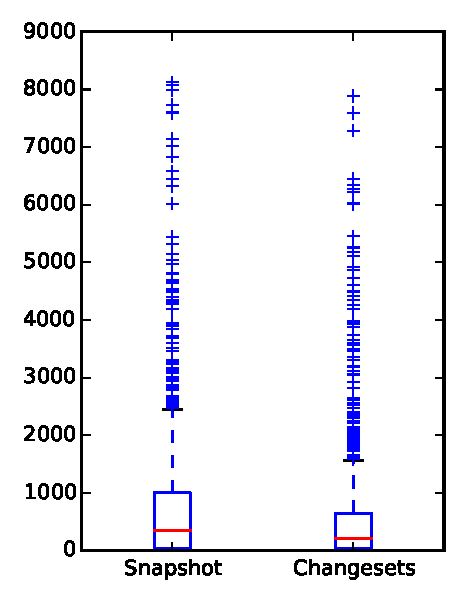
\includegraphics[width=0.24\textwidth]{figures/rq1-overall-class}
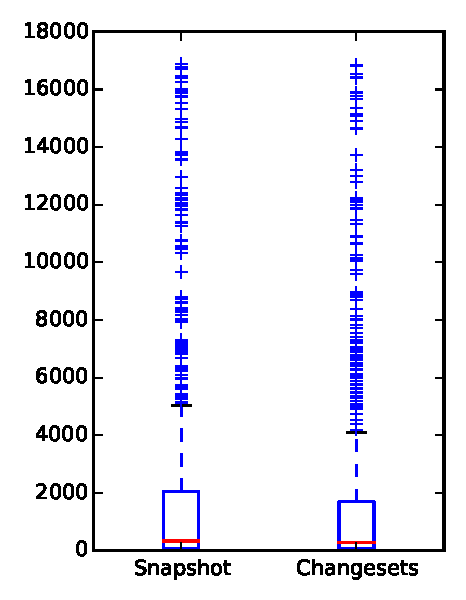
\includegraphics[width=0.24\textwidth]{figures/rq1-overall-method}
\caption{RQ1: Effectiveness measures for classes (left) and methods (right) across all 14 systems}
\label{fig:em}
\end{figure}

\begin{figure*}[t]
\centering
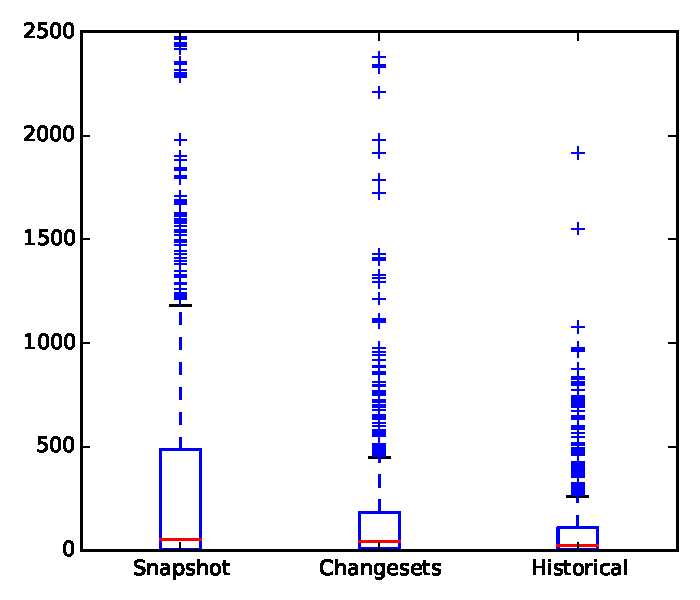
\includegraphics[width=0.36\textwidth]{figures/rq2-overall-class}
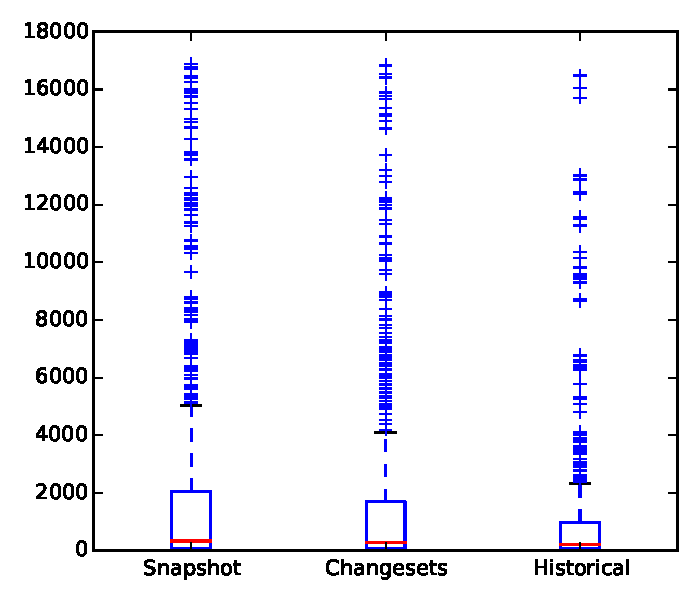
\includegraphics[width=0.36\textwidth]{figures/rq2-overall-method}
\caption{RQ2: Effectiveness measures for classes (left) and methods (right) across all 6 systems}
\label{fig:em6}
\end{figure*}

Figure~\ref{fig:em} shows the effectiveness measures for methods and classes
across all systems. The figure suggests that snapshot-based models and
changeset-based models have similar results overall with changesets performing
slightly better, but does not help to understand how each feature query performs
for each model.  With respect to RQ1, we will investigate the queries and
effectiveness measures between the batch snapshot and batch changesets in
detail.

For the 1214 successful queries of classes,
each query returns the same effectiveness measure 30 out of 1214 times, or about 2.5\% of the time.
Of these 30, 17 of them all return an effectiveness measure of 1 (the best possible measure).
For 178 queries (14.7\%), the effectiveness measure is within 10 ranks of each other.
For 356 queries (29.3\%), the effectiveness measure is within 50 ranks of each other.
The remaining 858 queries (70.6\%) perform noticibly different ($> 50$ ranks apart).

For the 629 successful queries of methods,
each query returns the same effectiveness measure 12 out of 629 times, or about 1.9\% of the time.
Of these 12, 7 of them all return an effectiveness measure of 1 (the best possible measure).
For 65 queries (10.3\%), the effectiveness measure is within 10 ranks of each other.
For 151 queries (24.0\%), the effectiveness measure is within 50 ranks of each other.
The remaining 478 queries (76.0\%) perform noticibly different ($> 50$ ranks apart).

Figure~\ref{fig:em6} shows the effectiveness measures for methods and classes
across the 6 systems considered in RQ2. The figure shows that the historical
simulation outperforms both batch evaluations, but does not help to understand
how each feature query performs for each model.  With respect to RQ2, we will
investigate the queries and effectiveness measures between the historical
simulation and the batch evaluations in detail.

For the 603 successful queries of classes,
each query returns the same effectiveness measure 8 out of 603 times, or about 1.3\% of the time.
Of these 8, 7 of them all return an effectiveness measure of 1 (the best possible measure).
For 111 queries (18.4\%), the effectiveness measure is within 10 ranks of each other.
For 230 queries (38.1\%), the effectiveness measure is within 50 ranks of each other.
The remaining 373 queries (61.9\%) perform noticibly different ($> 50$ ranks apart).

For the 595 successful queries of methods,
each query returns the same effectiveness measure 9 out of 595 times, or about 0.5\% of the time.
All 3 of these return an effectiveness measure of 1 (the best possible measure).
For 23 queries (3.9\%), the effectiveness measure is within 10 ranks of each other.
For 77 queries (12.9\%), the effectiveness measure is within 50 ranks of each other.
The remaining 518 queries (87.1\%) perform noticibly different ($> 50$ ranks apart).

\begin{comment}
\begin{table}[t]
\renewcommand{\arraystretch}{1.3}
\footnotesize
\centering
\caption{ArgoUML v0.26.2 Queries}
\begin{tabular}{r|p{0.8\linewidth}}
\toprule
Feature \# & Bag-of-words representation  \\
\midrule
5088       &

profiles (4),
xmi (3),
user (3),
profile (3),
write (3),
save (2),
files (2),
defined (2),
loaded (2),
impl (2),
mdr (2),
writer (2),
models (2),
able (1),
available (1),
implemented (1),
file (1),
model (1),
issue (1),
release (1),
aren (1),
using (1),
isn (1),
zargo (1),
creating (1),
removed (1),
configuration (1),
removing (1),
empty (1),
won (1),
seams (1),
persister (1),
usage (1),
simply (1),
written (1),
depend (1),
due (1),
configured (1),
deeper (1),
directories (1),
experimentally (1),
flag (1),
functionality (1),
persist (1),
prevents (1),
tackle (1),
unassigned (1),
wasn (1),
writing (1)

\\
5258       &

name (2),
classifier (2),
perspective (2),
collaboration (2),
rules (2),
explorer (1)

\\
\bottomrule
\end{tabular}
\label{table:argoumlqueries}
\end{table}



ArgoUML v0.26.2 feature 5258 has an effectiveness measure of 1 under the
snapshot-based model and 8138 under the changeset-based model, while feature
5088 had 1 under the changeset-based model and 124 under the snapshot-based
model.  Table~\ref{table:argoumlqueries} shows the bag-of-words representation
of each feature query.

Feature 5258 returns 3 related snapshot topics: 194 (58\%), 226 (18\%), and 464 (14\%).
The most related snapshots topics of the first relevant method at rank 1,
\texttt{GoClassifierToInstance.getRuleName()},
are also 194 (82\%), 226 (6\%), and 464 (4\%).
Hence, the snapshot model performs as expected.
Feature 5258 returns 2 related changeset topics: 250 (48\%) and 365 (43\%).
Unforunately, the first relevant method at rank 8138,
\texttt{GoClassifierToInstance.getRuleName()},
returns 2 different changeset topics: 432 (76\%) and 332 (17\%).
However, with the exception of changeset topic 432, the top words in these
topics are similar to that of the query. Changeset topic 432 appears to be a general
topic, consisting of words like ``jar'' (8\%), ``argouml'' (6\%), and ``org'' (5\%).

Feature 5088 returns 18 snapshot topics, with 3 highly ($> 10\%$) related: 281 (19\%), 283 (13\%), and 38 (11\%).
There are 6 snapshot topics for the first relevant method at rank 142,
\texttt{XmiWriterMDRImpl.write()},
and the highly related topics are 283 (56\%), 82 (16\%), and 41 (12\%).
We note that both each of these contain snapshot topic 283,
but the feature does not relate as highly to the topic as the method does.
We also note that the model seems confused about which topics are related to the feature.
Feature 5088 returns 19 changeset topics, with 3 highly related: 446 (21\%), 426 (12\%), and 472 (11\%).
The first relevant method at rank 1,
\texttt{testWritePreviouslyLoadedProfile()},
returns 10 changeset topics, with 3 highly related: 446 (47\%), 462 (15\%), and 426 (12\%).
7 out of the 10 changeset topics also appear in the 19 related to the feature.
Here, the changeset model was able to better discern which topics were related to the feature.

\end{comment}

\begin{comment}
\begin{table}[t]
\renewcommand{\arraystretch}{1.3}
\footnotesize
\centering
\caption{MuCommander v0.8.5 Queries}
\begin{tabular}{r|p{0.8\linewidth}}
\toprule
Feature \# & Bag-of-words representation \\
\midrule
37         &

        mac (3),
        menu (3),
        window (2),
        minimize (2),
        missing (2),
        zoom (2),
        application (1),
        mimic (1),
        options (1),
        standard (1)


\\
142       &

        java (7),
        drive (6),
        icons (3),
        button (3),
        popup (3),
        names (3),
        refresh (3),
        exception (2),
        hashtable (2),
        main (1),
        lang (1),
        mucommander (1),
        com (1),
        util (1),
        npe (1),
        pointer (1),
        run (1),
        thread (1),

\\
\bottomrule
\end{tabular}
\label{table:muqueries}
\end{table}



MuCommander v0.8.5 feature 37 has an effectiveness measure of 1 under the
snapshot-based model and 303 under the changeset-based model, while feature 142
had 1 under the changeset-based model and 536 under the snapshot-based model.
Table~\ref{table:muqueries} shows the bag-of-words representation of each
feature query.

\end{comment}

%%%% Awkwardddddddddd

In this study, we've also asked two research questions which lead to two
distinct comparisons.  First, we compare a batch TM-based FLT
trained on the changesets of a project's history to one trained on the snapshot
of source code entities.  Second, we compare a batch TM-based FLT
trained on changesets to a online TM-based FLT trained on the same
changesets over time.  Our results are mixed between the research questions,
hence we end up with four possible situations; we will now discuss each of these
situations in detail.

%
% Old blah-de-blah.
%
\subsubsection{Batch changesets are better than batch shapshot
\emph{and} batch changesets are better than changesets in the simulated environment}

% Snapshots < Changeset && Batch > Temporal
% Class
%   ArgoUML 0.24
%
% Method
%   ArgoUML 0.22

This situation occurs in
1 out of 6 systems at the class-level, and
1 out of 6 systems at the method-level.
We hypothesize that this is due to the nature of the batch evaluation versus the historical simulation.
In the batch evaluation, the model is trained on all data before being queried,
while in the historical simulation the model is trained on partial data before being queried.
This allows for the batch model to be more accurate because it is trained on more data
and reveals feature location research evaluations may not be accurately portraying
how an FLT would perform in a real scenario.

\subsubsection{Batch changesets are better than batch shapshot
\emph{and} changesets in the simulated environment are better than batch changesets}

% Snapshots < Changeset && Batch < Temporal
% Class
%   ArgoUML 0.22
%
% Method
%   JabRef
%   jEdit
%   muCommander

This situation occurs in
1 out of 6 systems at the class-level, and
3 out of 6 systems at the method-level.
We hypothesize that this is due to the same previous reason, but that
historical simulation more accurately captures the correct state of the system (i.e., the source code entities)
at the point in time when querying is done.
Since querying on the batch models is after the model is completely trained,
there may be source code entities that do not exist in the system anymore
that were at one time changed to complete a certain task.
Again, the historical simulation better captures this scenario.

\subsubsection{Batch snapshot are better than batch changeset
\emph{and} changesets in the simulated environment are better than batch changesets}

%  Snapshots > Changeset && Batch < Temporal
% Class
%   ArgoUML 0.26
%   JabRef
%   jEdit
%   muCommander
%
% Method
%   ArgoUML 0.24
%   ArgoUML 0.26

This situation occurs in
4 out of 6 systems at the class-level, and
2 out of 6 systems at the method-level.
Similarly, this could be because of how the models are trained.
Although the batch changesets performed worse in both cases, it does
improve during historical simulation.
This does not mean that changesets are bad, but more accurately model
the system over time.

\subsubsection{Batch snapshot are better than batch changeset
\emph{and} batch changesets are better than changesets in the simulated environment}

% Snapshots > Changeset && Batch > Temporal
% Class
%
% Method
%
We note that this situation never occurs.
This also supports the hypothesis that historical simulation more accurately portrays the system over time.
However, we cannot conclude this without also historically simulating snapshot TM-based FLTs.


\section{Threats To Validity}
\label{sec:threats}
% vim:syntax=tex


\begin{figure}[t]
\footnotesize

{\bf bookkeeper-server.src.main.java.}org.apache.bookkeeper.bookie.Bookie

{\bf bookkeeper-server.src.main.java.}org.apache.bookkeeper.bookie.EntryLogger

{\bf bookkeeper-server.src.test.java.}org.apache.bookkeeper.bookie.LedgerCacheTest

\caption{Corrected BookKeeper goldset for issue \#10. Bold text denotes the portion removed.}
\label{fig:goldsetfix}
\vspace{-15pt}
\end{figure}


Our study has limitations that impact the validity of our findings,
as well as our ability to generalize them.
We describe some of these limitations and their impacts.

Threats to construct validity concern measurements accurately reflecting the features of interest.
A possible threat to construct validity is our benchmarks.
Errors in the datasets could result in inaccurate effectiveness measures.
The datasets were produced by other researchers, are publicly available,
and have been used in previous research~\cite{Dit-etal:2013, Revelle-etal:2010, Moreno-etal:2014}.
While both datasets extracted source code entities automatically from changesets and patches,
previous work shows this approach is on par with manual extraction~\cite{Corley-etal:2011}.

Additionally, we found errors within the datasets themselves that would be a threat to construct validity.
In particular, the Moreno et al. dataset included classes that had package names that were not valid.
Figure~\ref{fig:goldsetfix} describes the classes reported in the dataset and the corrected classes used in our dataset.
We make the assumption that the authors of this dataset used the directory structure of the project to build the package names.
Manual correction was required as our tool parses the files and uses the package name given in the source file, not the directory structure.

Threats to internal validity include possible defects in our tool chain and possible errors
in our execution of the study procedure,
the presence of which might affect the accuracy of our results and the conclusions we draw from them.
We controlled for these threats by testing our tool chain and by assessing the quality of our data.
Because we applied the same tool chain to all subject systems, any errors are systematic and are unlikely
to affect our results substantially.

Another threat to internal validity pertains to the value of parameters such as $K$ that we selected for all models trained.
We decided that the changeset and snapshot models should have the same parameters to help facilitate evaluation and comparison.
We argue that our study is not about selecting the best parameters,
but to show that our changeset TM-based FLT approach is reasonable.

Threats to external validity concern the extent to which we can generalize our results.
The subjects of our study comprise fourteen open source projects in Java,
so we cannot generalize our results to systems implemented in other languages.
However, the systems are of different sizes, are from different domains, and
have characteristics in common with those of systems developed in industry.



\section{Conclusions \& Future Work}
\label{sec:conclusion}
% vim:syntax=tex

In this paper we conducted a study on modeling the topics of changesets in
comparison to the traditional snapshot approach.  We use latent Dirichlet
allocation (LDA) to extract linguistic topics from changesets and snapshots
(releases).

We addressed two research questions regarding the performance of a TM-based FLT
trained on changesets.  First, we compare a batch TM-based FLT trained on the
changesets of a project's history to one trained on the snapshot of source code
entities.  We found that changesets can perform as well as or better than
snapshots.  Second, we compare a batch TM-based FLT trained on changesets to
a historical simulation of a TM-based FLT trained on the same changesets over
time.  We show that the historical simulation more accurately portrays how a FLT
would execute in a real environment.

Our results encourage the idea that there is still much to explore in the area
of feature location. What other untapped resources might be available? We show
changesets are yet another viable resource researchers and practitioners should
be taking advantage of for the feature location task.  Our results also show
that research remains not only in improving accuracies of FLTs, but also in
solving the practical aspects of building FLTs that are robust \emph{and} agile
enough to keep up with fast-changing software.

Future work includes deploying this appoach in a development environment.  Since
the source code to our approach is online, we encourage other researchers to
investigate this future work as well.  We also would like to expand the simulation 
parts of this study to include both snapshots and changesets.  It would be
particularly useful to compare results between batch snapshots and simulated
snapshots. 

Additional future work exists in regard to configuration. In a changeset
it may be desirable to parse further for source code entities using
island grammar parsing~\cite{Moonen:2001}.  It may also be desirable to
only use portions of the changeset, such as only using added or removed
lines, or extracting changes between the abstract syntax
trees~\cite{Fluri-etal:2007}. Most importantly, like previous
work~\cite{Biggers-etal:2014}, it would be wise to further investigate
the effects of the two online LDA variables, $\tau_0$ and $\kappa$.  We
leave these options for future work.



\section*{Acknowledgment}
%We thank the anonymous reviewers for their insightful comments and helpful suggestions.
This material is based upon work supported
by the National Science Foundation under Grant No.\ 1156563. % REU grant for KLK

\newpage
\bibliographystyle{IEEEtran}
\bibliography{paper}

\end{document}
